\section{Zbiór danych}

W~projekcie wykorzystana została baza danych \textbf{Fruits-360} \cite{fruits-360}, która inkorporuje zbiór ponad 90 tys. zdjęć owoców podzielonych na 131 klas. Zdjęcia dostarczone są w~formacie JPEG, a~ich wielkość została ustandaryzowana do wymiaru $100\times100$ pikseli. Warto nadmienić, że różne warianty tych samych gatunków owoców zostały umieszczone w~oddzielnych klasach. Dane zostały podzielone przez autorów na dwa podzbiory: \textit{Training} (67692 zdjęć) i \textit{Test} (22688 zdjęć).

\subsection{Potok}

\vspace{0.5cm}
\begin{figure}[h]
    \centering
    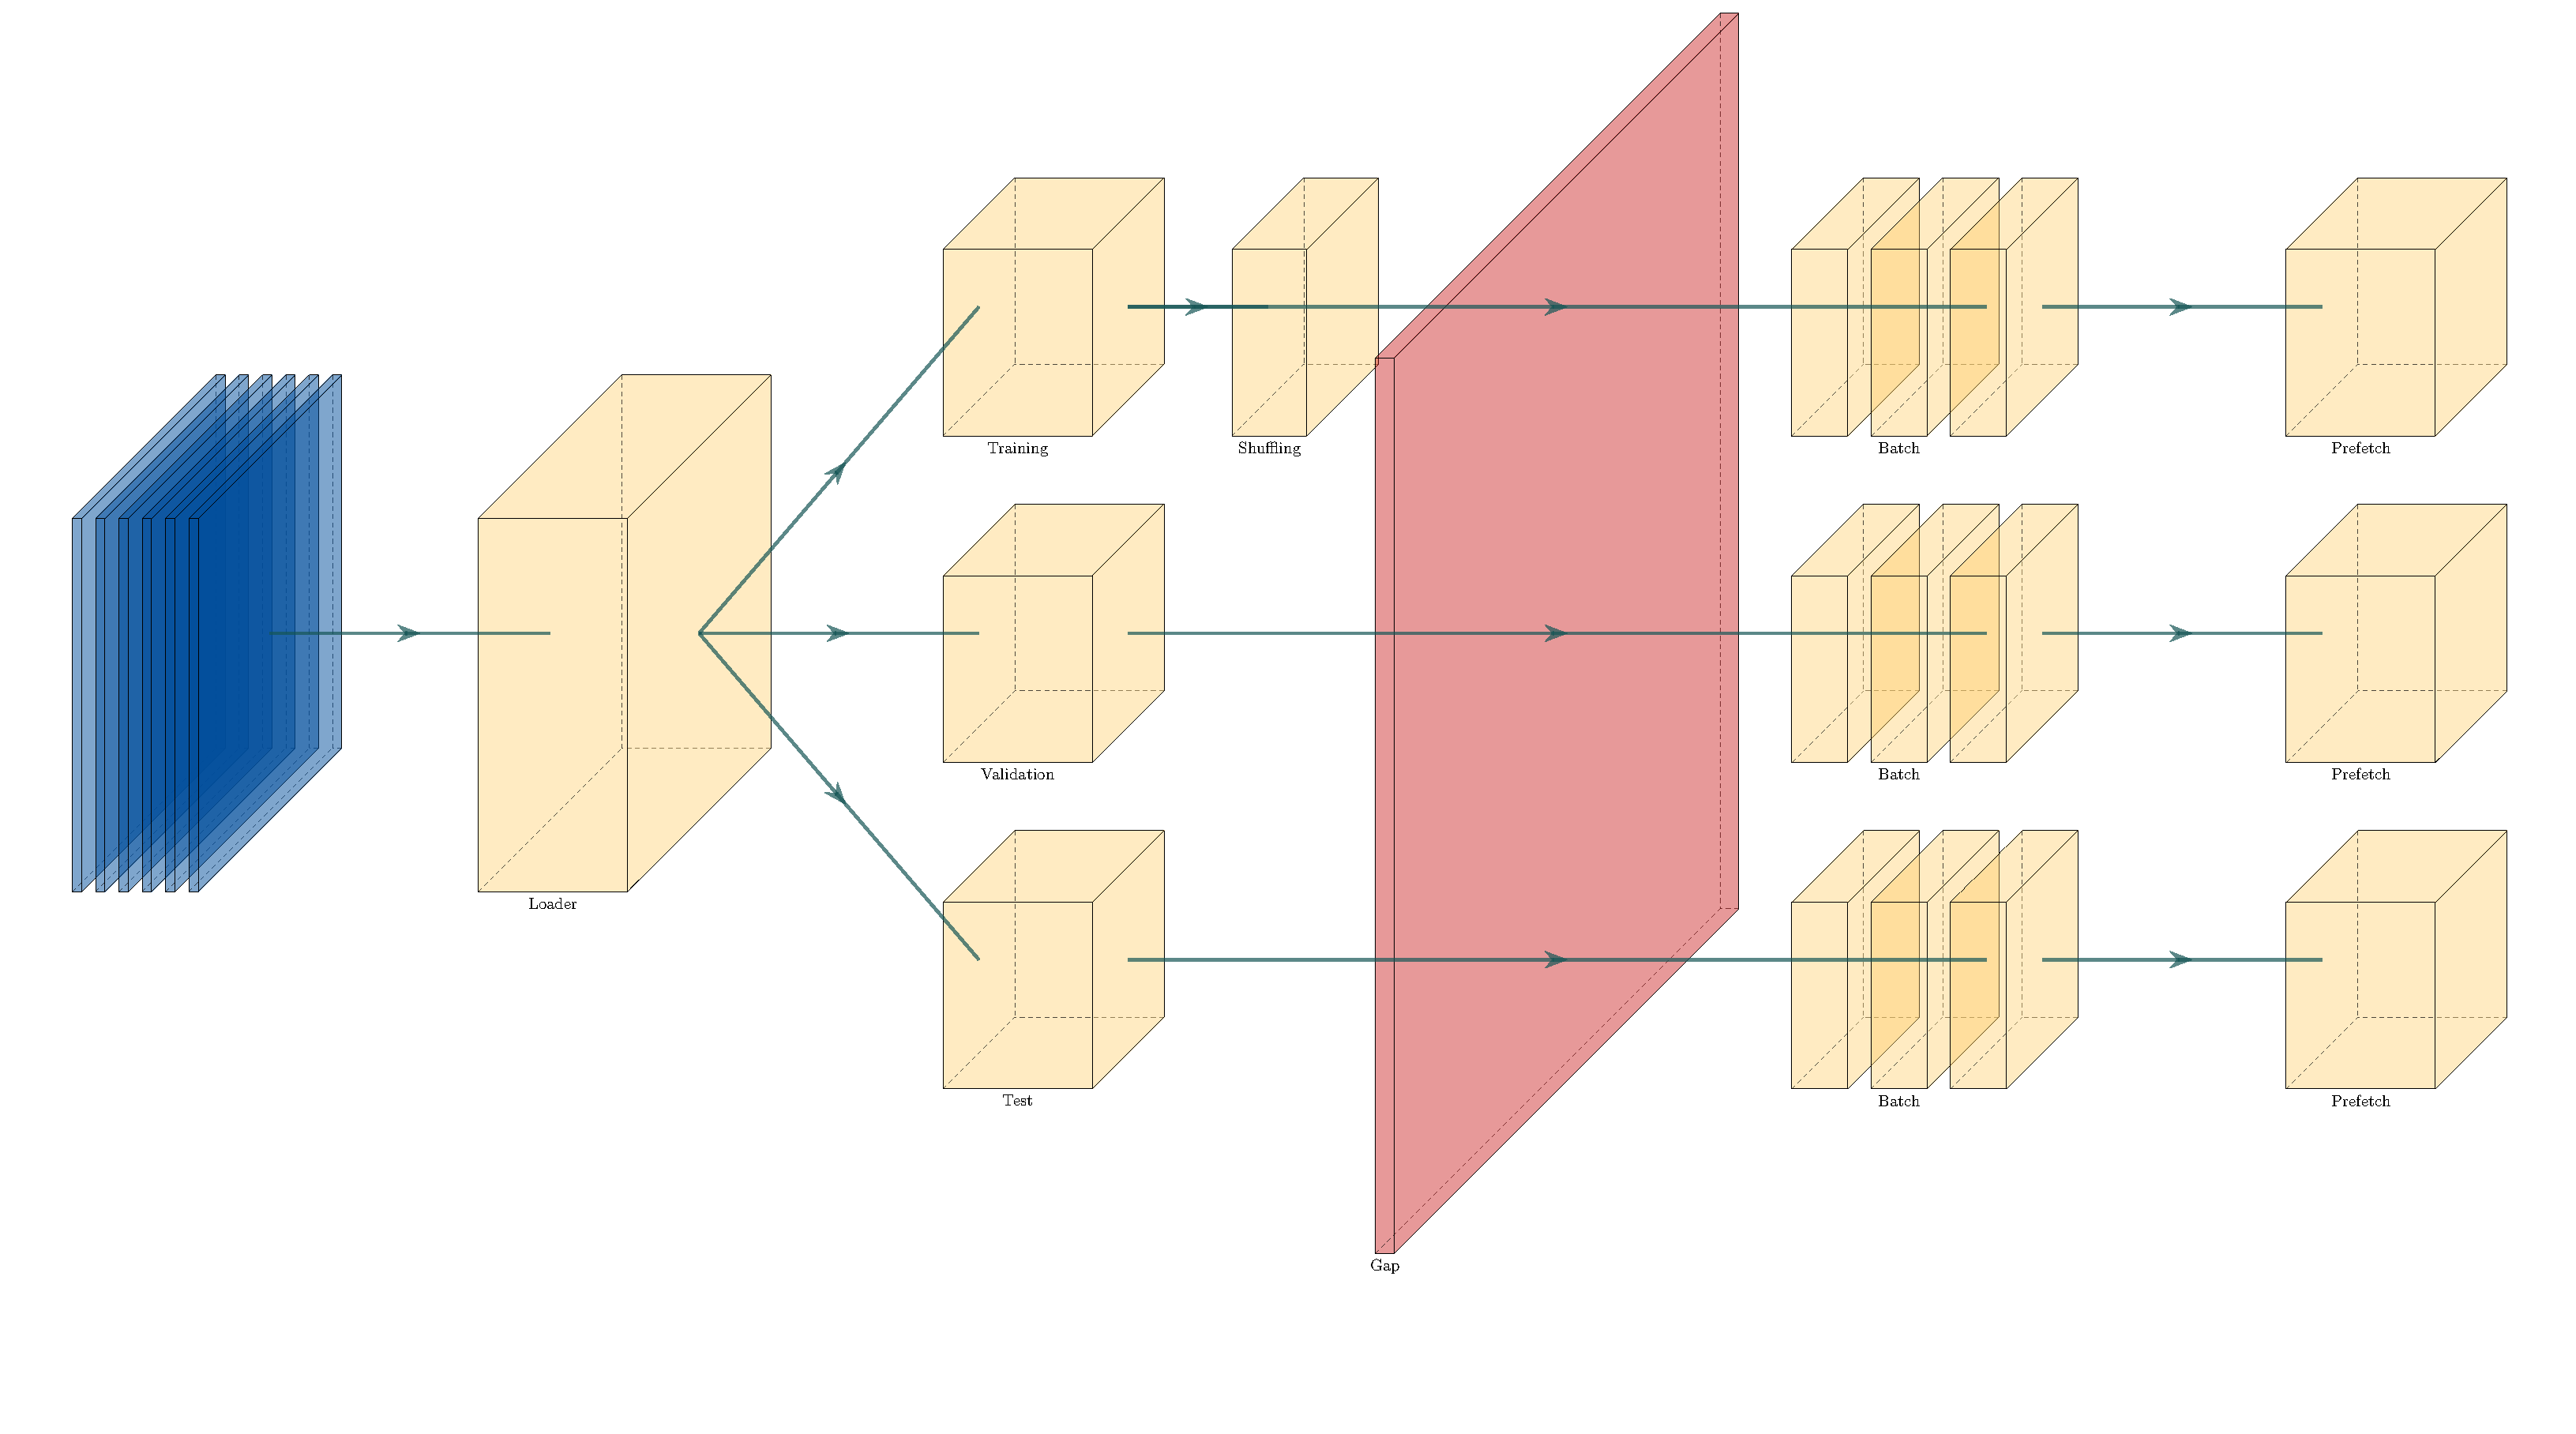
\includegraphics[scale=0.2]{img/pipe.pdf}
    \label{pipe_img}
    \caption{Struktura potoku danych wejściowych}
\end{figure}
\vspace{0.5cm}

Prace nad projektem rozpoczęto od wyboru bibliotek dostarczających zestaw podstawowych narzędzi uczenia maszynowego. Decyzja padła na popularny framework \textit{Tensorflow}, dzięki któremu możliwe było przygotowanie wygodnego, wysoce konfigurowalnego potoku danych wejściowych. Wykorzystanie \textit{tf.data} API pozwoliło na dynamiczne ładowanie danych do pamięci, co znacznie zredukowało jej zużycie  w~procesie uczenia. Możliwość zrównoleglenia tego procesu względem obliczeń wykonywanych na procesorze graficznym usunęła występujące początkowo wąskie gardło w~postaci procesu przenoszenia danych z~pamięci operacyjnej do VRAMu. Całość rozwiązania została zamknięta w~postaci klasy, której parametry mogłą być ustalane z~poziomu plików konfiguracyjnych. Takie podejście wyeliminowało potrzebę ingerowania w~kod źródłowy na etapie eksploatacji potoku. 

Rys. \ref{pipe_img} przedstawia graficzną reprezentację przepływu danych. Na wejściu następuje przydzielenie danych do trzech zbiorów. Podzbiór \textit{Training} jest w całości wykorzystywany jako zbiór treningowy. Z~kolei \textit{Test} \textbf{dzielony jest w~stosunku $1:1$} na dane walidacyjne i~testowe. W~kolejnym kroku nastepuje losowe przemieszanie danych treningowych. Obszar zaznaczony na rysunku na czerwono oznacza lukę. W~tym miejscu na zbiory można nałożyć arbitralne modyfikacje, co wykorzystywane jest na etapie augmentacji. Następnie wszystkie zbiory zostają podzielone na porcje (ang. \textit{mini-batches}). Ostatecznie część danych zostaje pobrana do bufora w~pamięci operacyjnej (faza \textit{prefetch}).
\subsection{Augmentacja}

